\chapter{実験による提案手法の評価}
\thispagestyle{empty}
\label{chap5}
\minitoc

\newpage
%%%%%%%%%%%%%%%%%%%%%%%%%%%%%%%%%%%%%%%%%%%%%%%%%%%%%%%%%%%%%%%%%%%%%%%%%%%%%%%
%==============================================================================
% 5.1
%==============================================================================
\section{はじめに}

本章では,提案手法による位置姿勢推定の計算時間,精度,ロバスト性について評価する.

まず5.2節にて,実験の概要について述べる.

次に5.3節にて,シミュレーション環境における実験について述べる.

最後に5.4節にて,実環境における実験について述べる.

\clearpage
%==============================================================================
% 5.2
%==============================================================================
\section{実験の概要}

本研究では,シミュレーション環境と実環境の2つの環境において位置姿勢推定を行った.
シミュレーション環境における実験では,3DCGソフトウェアBlender\mbox{\cite{Blender}}を用いて任意の位置姿勢において全天球カメラ画像を生成し,生成された全天球カメラ画像を入力画像として位置姿勢推定を行った.環境中の5地点において,姿勢を20回変化させて計100枚の全天球画像を生成し,位置姿勢推定を行った.
実環境における実験では,異なる位置姿勢の5地点において撮影した全天球カメラ画像を入力画像として位置姿勢推定を行った.

\clearpage
%==============================================================================
% 5.3
%==============================================================================
\section{シミュレーション環境における提案手法の評価}

シミュレーション環境における実験では,環境中の様々な位置姿勢において位置姿勢推定を行い,計算時間と推定精度を評価することで,本手法の有効性を検証した.

\subsection{実験の設定}

シミュレーション環境における実験で用いた3次元モデルを図\ref{fig:env_model}に示す.
また,このモデルをもとに作成したラインマップを図\ref{fig:env_line}に示す.
環境の大きさは,幅7.9m,奥行き2.8m,高さ2.9mであった.
環境中の5つの異なる地点において,それぞれの位置で姿勢を変えながら20通りの位置姿勢をサンプルし,サンプルした位置姿勢を真値として解像度600$\times$300 pix の全天球カメラ画像を生成し位置姿勢推定を行った.
姿勢変化は,$\phi$と$\theta$がそれぞれ-10~10 degの範囲でランダムな値とし,$\psi$を0 degから18 degずつ増やしていくことで,各地点において20通りの異なる姿勢の画像を生成した.
また,各地点の座標は\ref{tab:simu_pos}に示す通りである.
\\

\begin{figure}[b]
 \begin{center}
 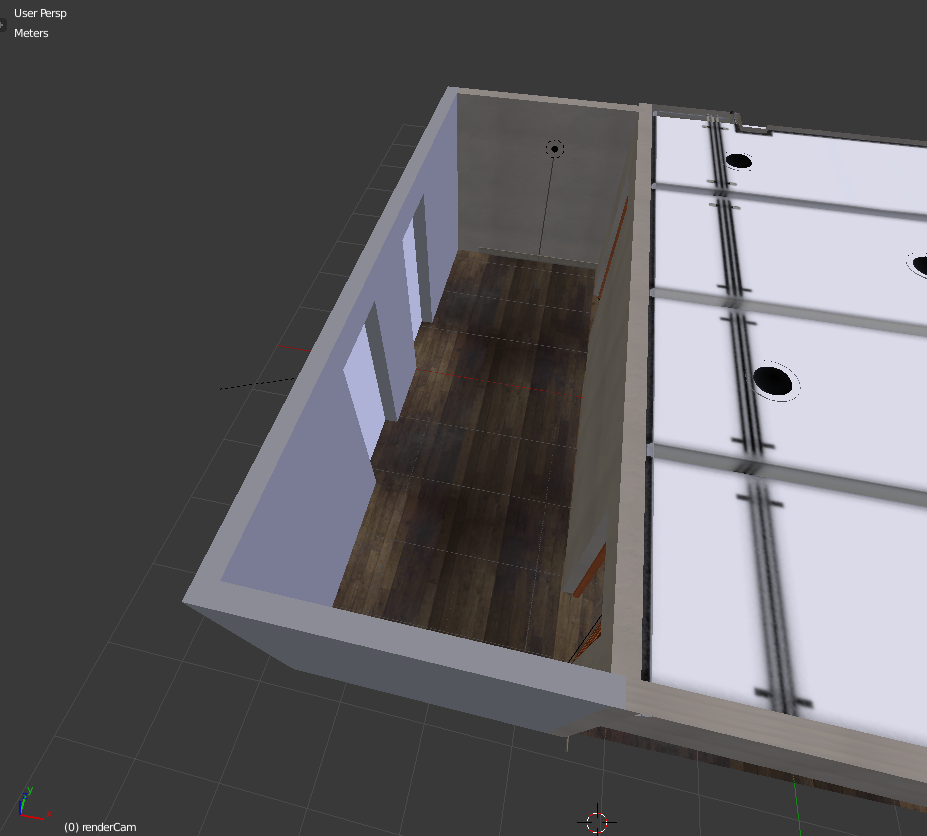
\includegraphics[width=0.6\columnwidth]{./chap5/fig/blender_room_2.png}
 \caption{シミュレーション環境の3次元モデル}
 \label{fig:env_model}
 \end{center}
 \vspace{-5mm}
\end{figure}

\begin{figure}[tb]
 \begin{center}
 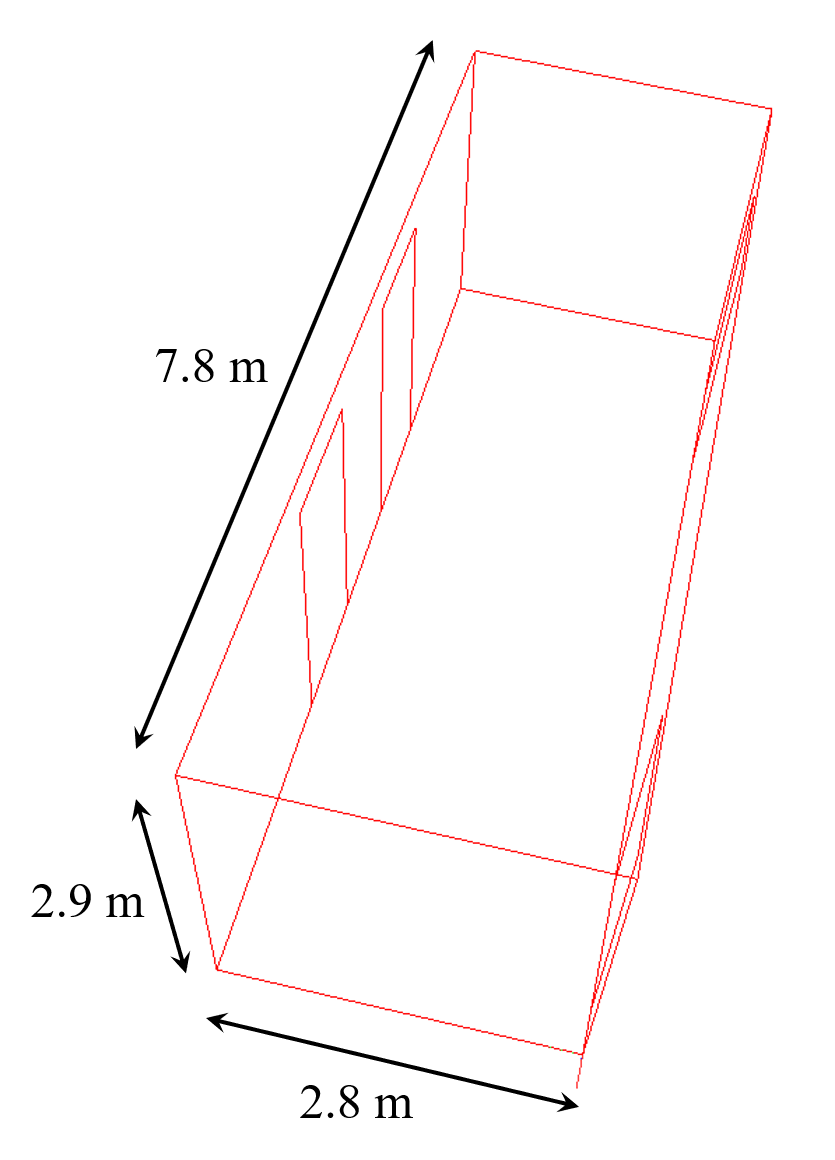
\includegraphics[width=0.5\columnwidth]{./chap5/fig/linemap.png}
 \caption{シミュレーション環境のラインマップ}
 \label{fig:env_line}
 \end{center}
 \vspace{-5mm}
\end{figure}

\begin{table}[htb]
 \begin{center}
 \caption{シミュレーション環境におけるカメラの位置}
  \begin{tabular}{c||c|c|c} \hline
    地点 & $x$ m & $y$ m & $z$ m \\ \hline \hline
     1 & 2.5 & 1.2 & 1.2  \\ 
     2 & 5.5 & 1.2 & 1.2  \\ 
     3 & 3.5 & 1.4 & 1.2  \\
     4 & 2.5 & 1.6 & 1.2  \\
     5 & 5.5 & 1.6 & 1.2  \\ \hline
  \end{tabular}
 \label{tab:simu_pos}
 \end{center}
\end{table}

取得した画像の例を図\ref{fig:input_simu}に示す.

\begin{figure}[tb]
 \begin{center}
 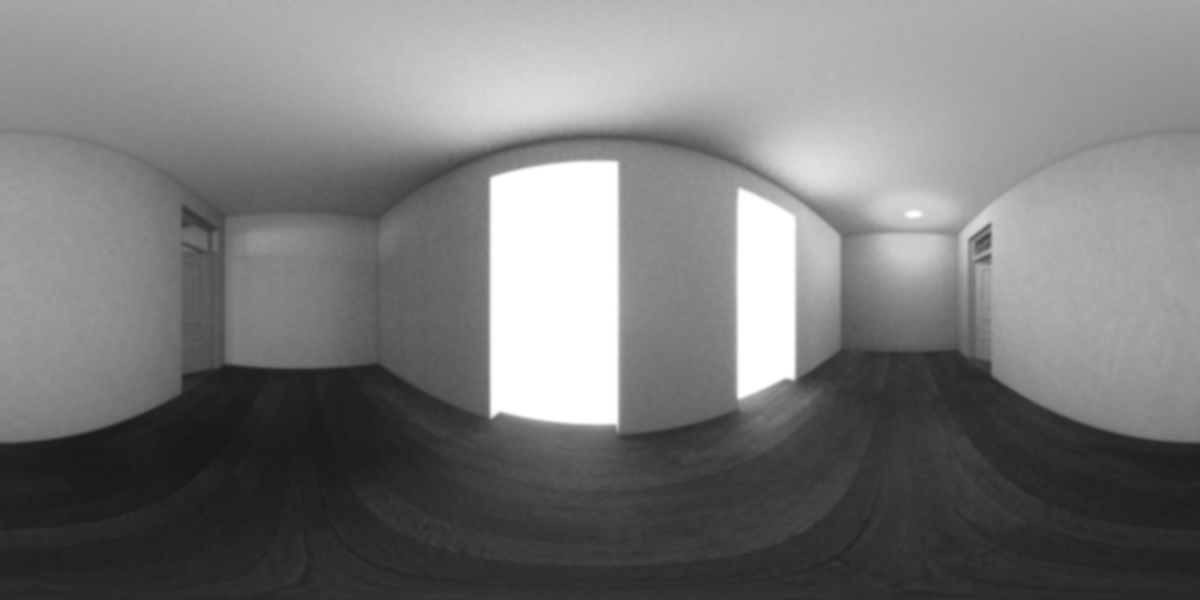
\includegraphics[width=0.7\columnwidth]{./chap5/fig/blurred_image.png}
 \caption{シミュレーション環境での実験における入力画像の例}
 \label{fig:input_simu}
 \end{center}
 \vspace{-5mm}
\end{figure}


\clearpage
\subsection{結果および考察}

結果は位置姿勢の推定誤差で評価する.
このとき,位置の推定誤差$\it{P}_e$は,$x$軸方向の誤差を$x_e$,$y$軸方向の誤差を$y_e$,$z$軸方向の誤差を$z_e$とすると,
\begin{equation}
P_e = \sqrt{x_e^2+y_e^2+z_e^2},
\end{equation}
によって,ユークリッド距離で表す.また,姿勢の誤差$\it{O}_e$は,オイラー角をクォータニオンを用いて1軸の回転角に変換して表す.
オイラー角における$x$軸回りの回転角の誤差を$\phi_e$,$y$軸回りの回転角の誤差を$\theta_e$,$z$軸回りの回転角の誤差を$\psi_e$とすると,
\begin{equation}
O_e = 2\cos^{-1}\left(C_1C_2C_3-S_1S_2S_3\right),
\end{equation}
によって計算される.ここで,
\begin{eqnarray}
  C_1 & = & \cos\left(\frac{\phi_e}{2}\right), \nonumber \\
  C_2 & = & \cos\left(\frac{\theta_e}{2}\right), \nonumber \\
  C_3 & = & \cos\left(\frac{\psi_e}{2}\right), \nonumber \\
  S_1 & = & \sin\left(\frac{\phi_e}{2}\right), \nonumber \\
  S_2 & = & \sin\left(\frac{\theta_e}{2}\right), \nonumber \\
  S_3 & = & \sin\left(\frac{\psi_e}{2}\right),
\end{eqnarray}
である.

\clearpage
\subsubsection*{計算時間}
100回の推定における位置姿勢推定の平均計算時間は,3.3$\pm$2.3秒であった.
1枚の画像の位置姿勢推定を行うのに20~30分程度要する従来手法\mbox{\cite{Goto2018}}と比べて大幅に計算時間が短縮されていることが確認できた.

\subsubsection*{推定精度}
100回の推定における位置姿勢推定の平均誤差は,位置の平均誤差が0.50$\pm$0.47m,姿勢の誤差が3.4$\pm$5.5degであった.$\pm$は標準偏差を表す.
\\

地点ごとの位置の推定誤差の平均と姿勢の推定誤差の平均をそれぞれ図\ref{fig:result1},図\ref{fig:result2}に示す.
\\

\begin{figure}[b]
 \begin{center}
 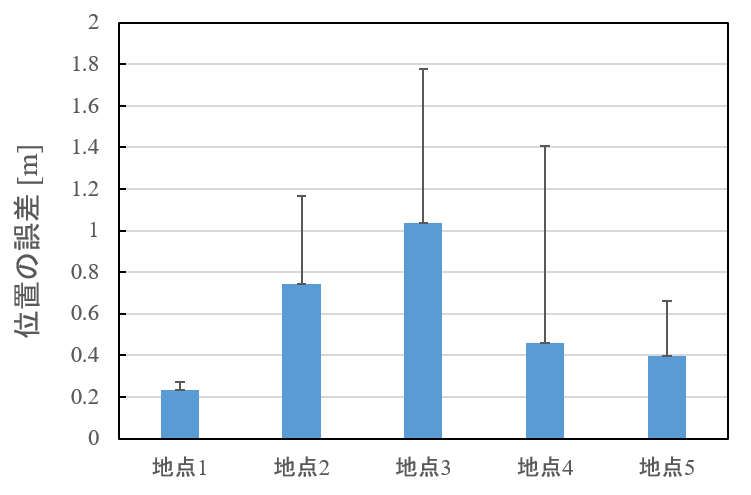
\includegraphics[width=0.7\columnwidth]{./chap5/fig/result1.png}
 \caption{位置推定の誤差分布}
 \label{fig:result1}
 \end{center}
 \vspace{-5mm}
\end{figure}

\begin{figure}[tb]
 \begin{center}
 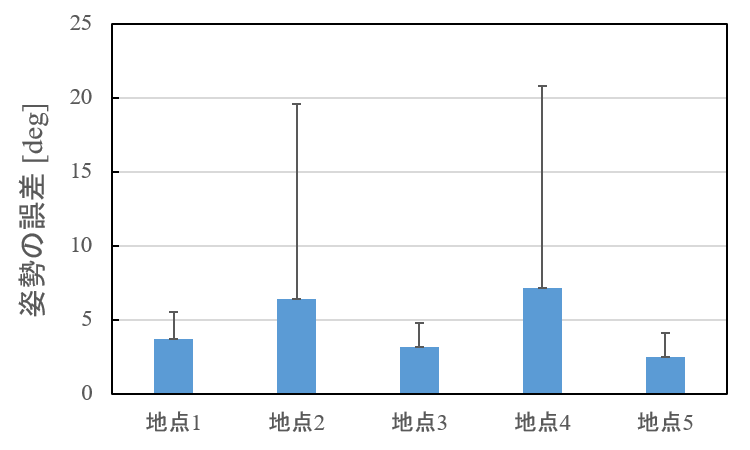
\includegraphics[width=0.7\columnwidth]{./chap5/fig/result2.png}
 \caption{姿勢推定の誤差分布}
 \label{fig:result2}
 \end{center}
 \vspace{-5mm}
\end{figure}

以上により,シミュレーション環境での実験において,要求仕様を満たす計算時間で推定に成功し,本手法の有効性を確認することができた.

\clearpage
%==============================================================================
% 5.4
%==============================================================================
\section{実環境における提案手法の評価}

本節では,実環境における実験について述べる.
シミュレーション環境における実験では,3次元モデルから直接映像を生成するため,3次元モデルと画像における直線の分布に誤差はないと考えられる.
一方で,実環境においては,壁に貼ってあるポスターや,壁や三脚の影など,3次元モデルには存在しない直線が画像に映ることも考えられる.
よって,実環境においても本手法の有効性を確認する必要がある.

\vspace{\baselineskip}
実環境における実験では,\mbox{\cite{Goto2018}}で使用されたデータを用いて実験を行い,計算時間と推定精度を比較した.


\subsection{実験の設定}

全天球カメラ画像は,表\ref{tab:spec}に示す仕様・スペックのRICOH THETA Sを用いて取得されたものである.


\begin{table}[htb]
 \begin{center}
 \caption{全天球カメラの仕様・スペック}
  \begin{tabular}{c|c} \hline
    製品名 & THETA S \\ 
    解像度 & 5,376$\times$2,688 pix \\ 
    接続方式 & Micro USB 端子,HDMI-Micro端子 \\ 
    サイズ & 44mm(幅)$\times$130mm(高さ)$\times$ 22.9mm(奥行き) \\
    重量 & 約125g \\ \hline
  \end{tabular}
 \label{tab:spec}
 \end{center}
\end{table}

各画像の位置姿勢の真値を表\ref{tab:real_pos}に,それぞれの画像を図\ref{fig:input_real}に示す.


\begin{table}[htb]
 \begin{center}
 \caption{実環境におけるカメラの位置姿勢の真値}
  \begin{tabular}{c||c|c|c|c|c|c} \hline
    地点 & $x$ m & $y$ m & $z$ m & $\phi$ deg & $\theta$ deg & $\psi$ deg \\ \hline \hline
     1 & 2.66 & 3.85 & 1.15 & 3.1 & 0.7 & -5.2  \\ 
     2 & 4.98 & 3.79 & 1.17 & 2.4 & 1.6 & 2.4  \\ 
     3 & 3.42 & 2.62 & 1.16 & 1.7 & 1.3 & -19.6  \\
     4 & 4.58 & 3.42 & 0.85 & -0.6 & -1.9 & 134.2  \\
     5 & 2.95 & 3.61 & 0.83 & 1.4 & 1.8 & -23  \\ \hline
  \end{tabular}
 \label{tab:real_pos}
 \end{center}
\end{table}


\setlength
\subfigcapskip{-0.6ex}
\begin{figure}[b]
	%\vspace{-10mm}
	\begin{center}
		\subfigure[地点1]{
		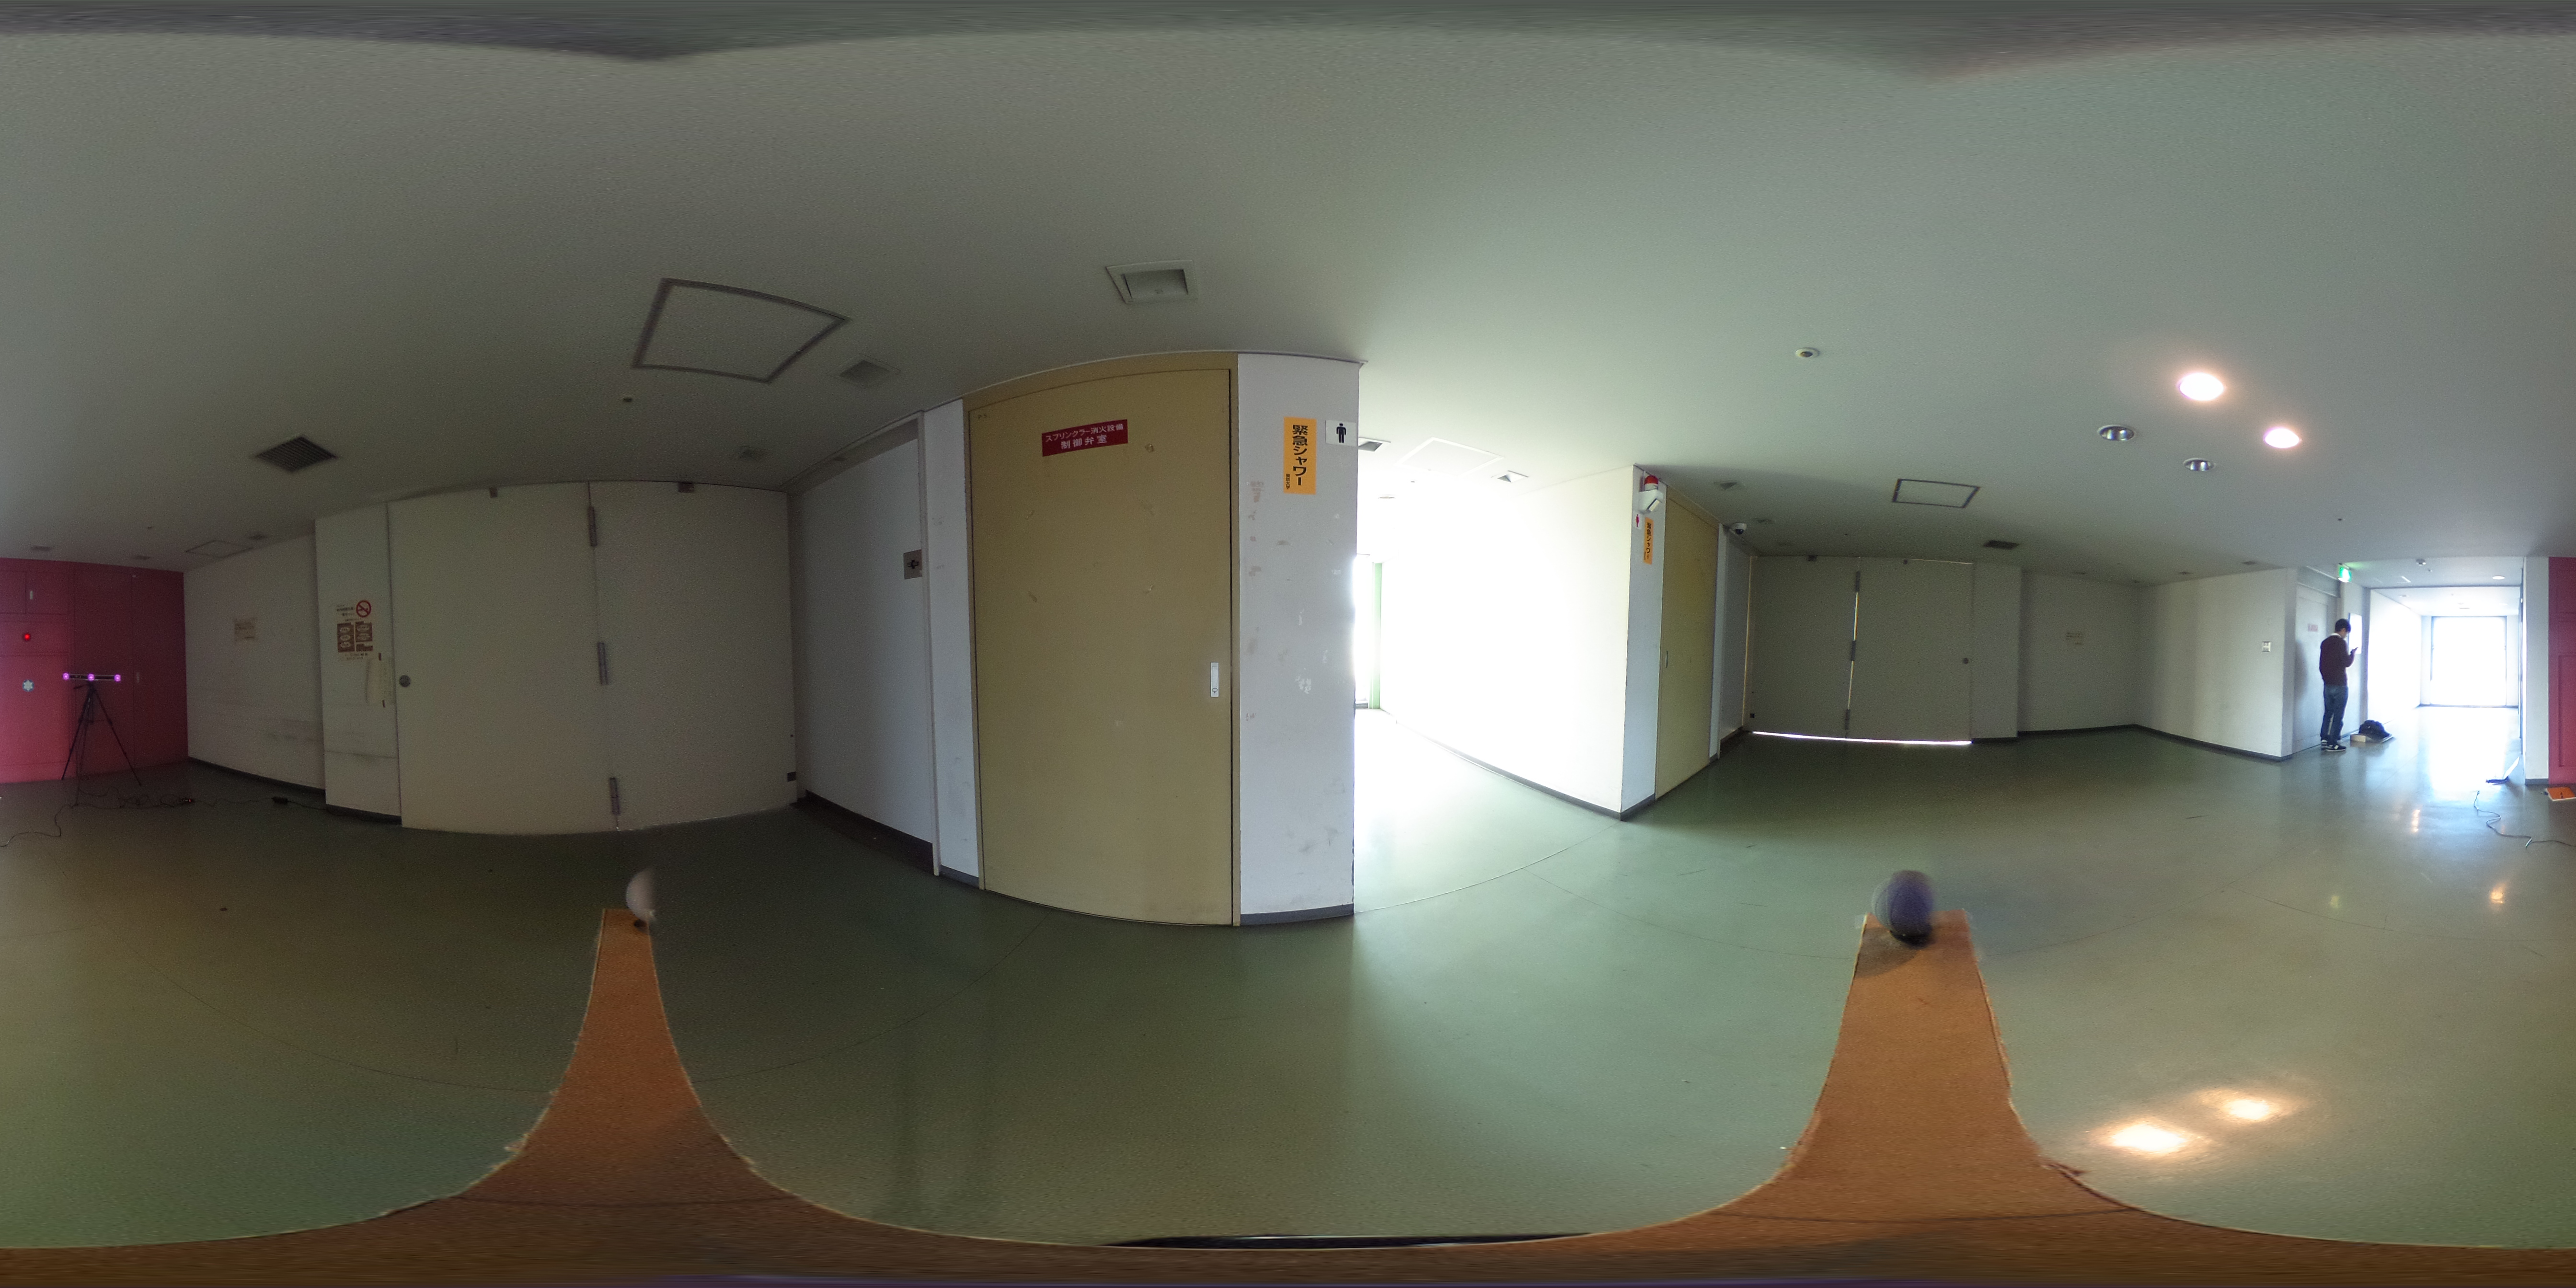
\includegraphics[clip,width=0.45\columnwidth]{./chap5/fig/1.jpg}}
		%\vspace{-5mm}
		\subfigure[地点2]{
		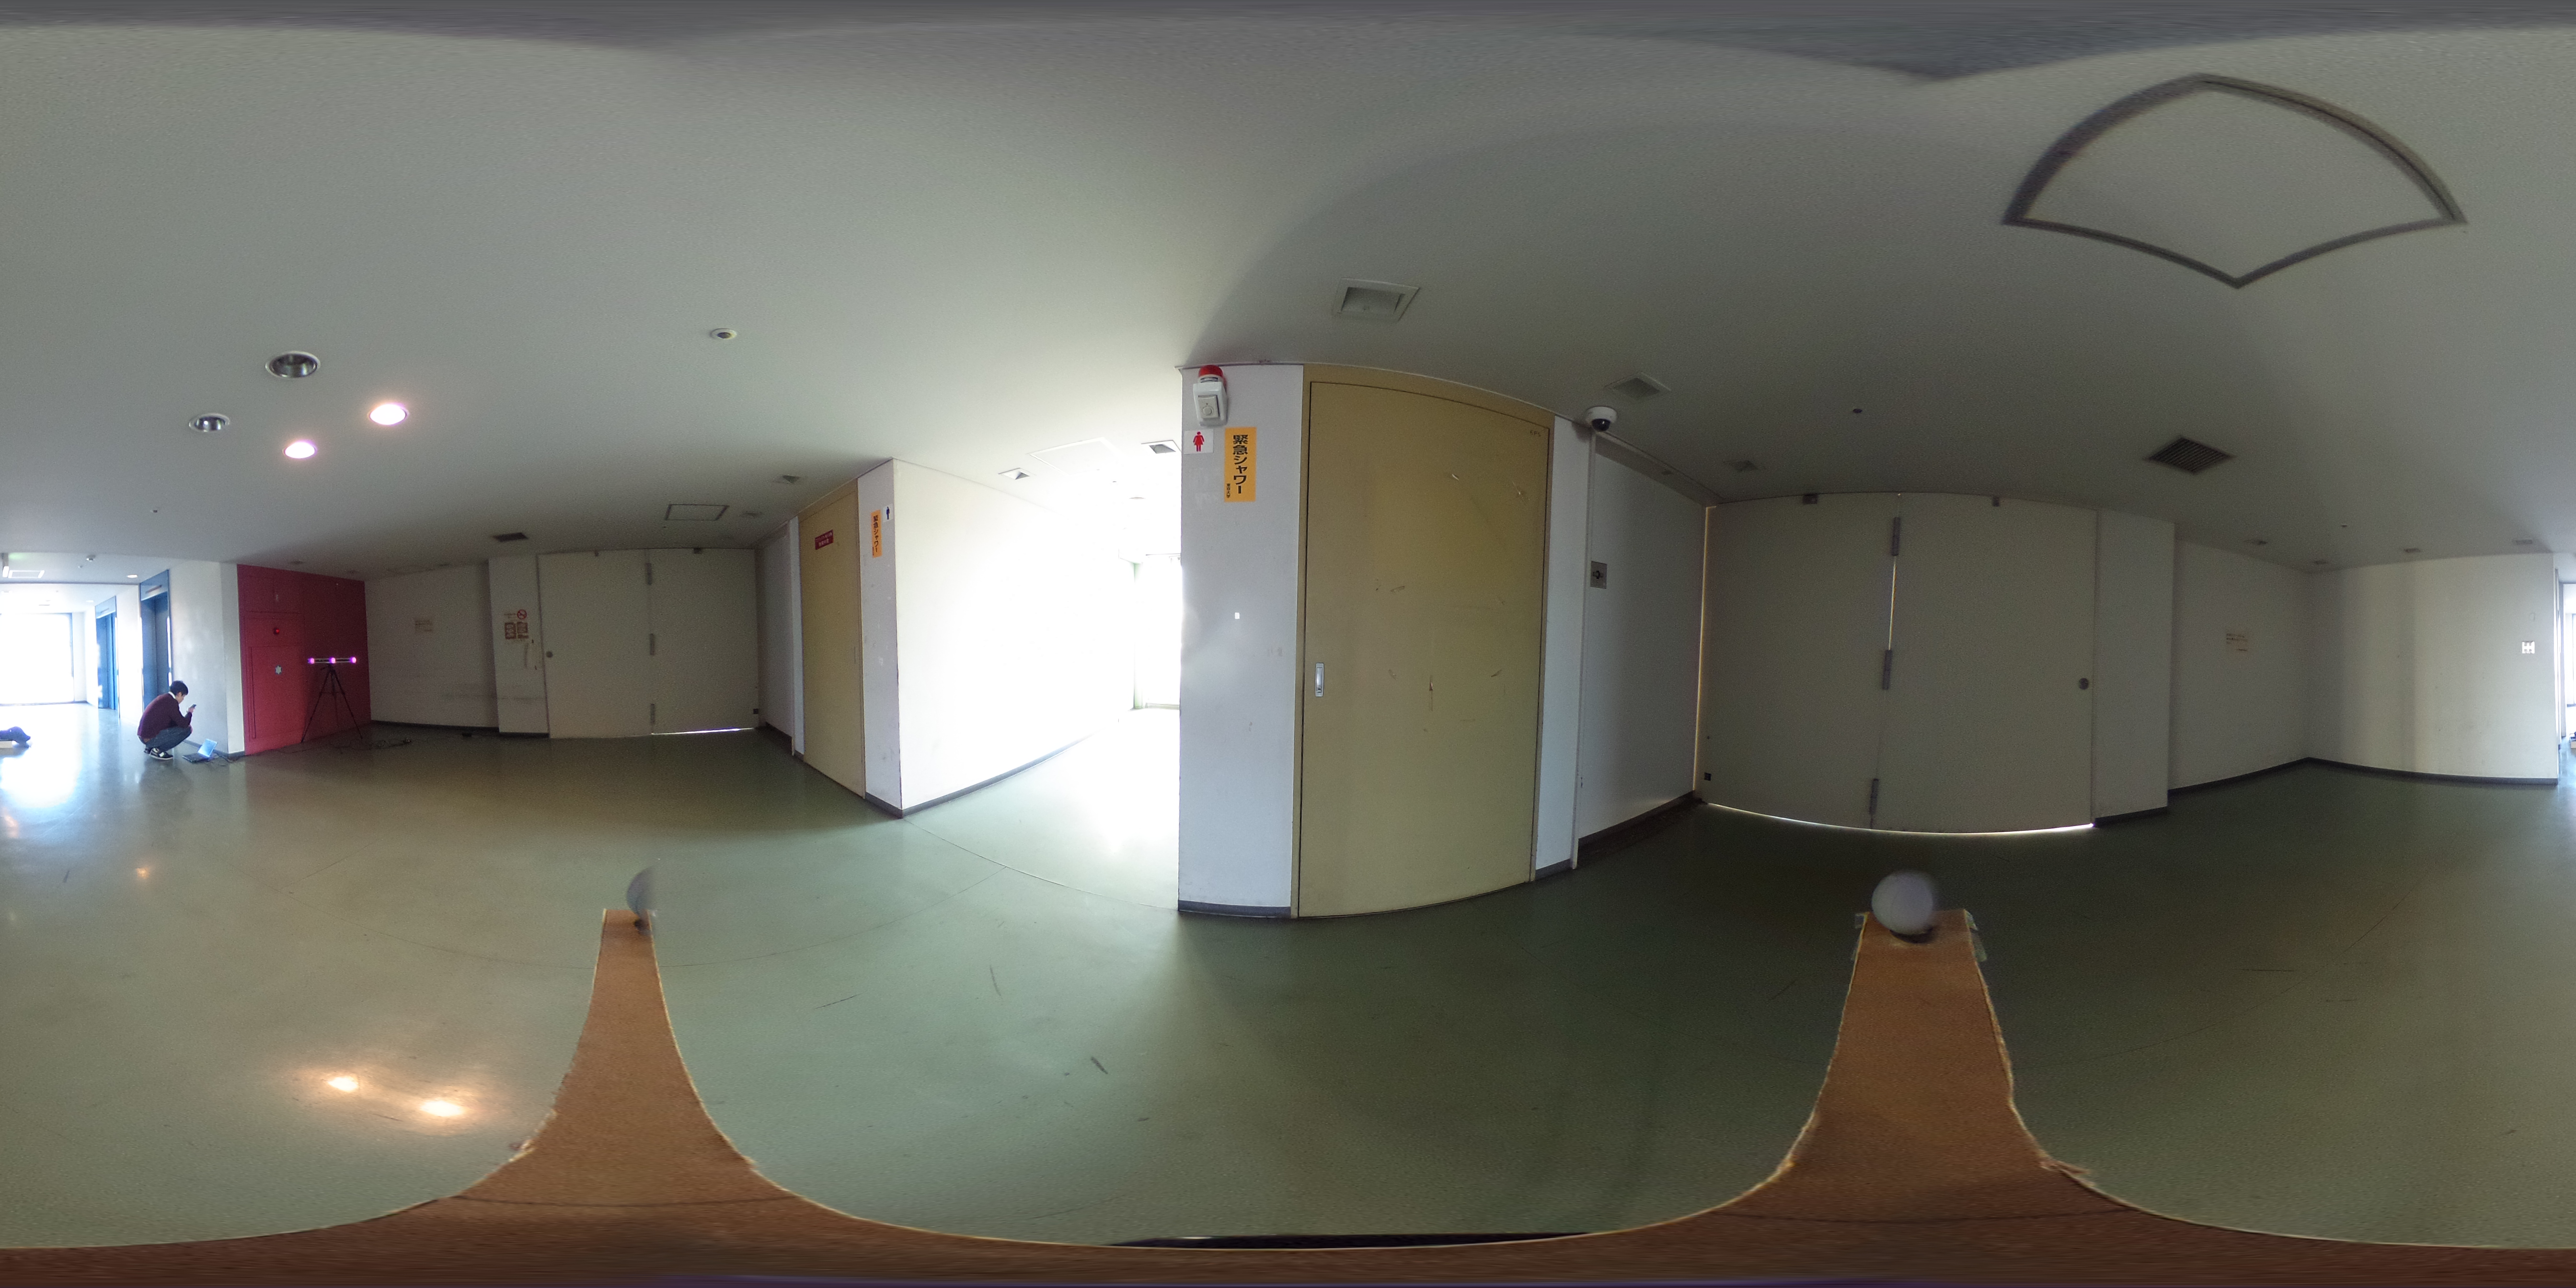
\includegraphics[clip,width=0.45\columnwidth]{./chap5/fig/2.jpg}}\\
		%\vspace{-5mm}
		\subfigure[地点3]{
		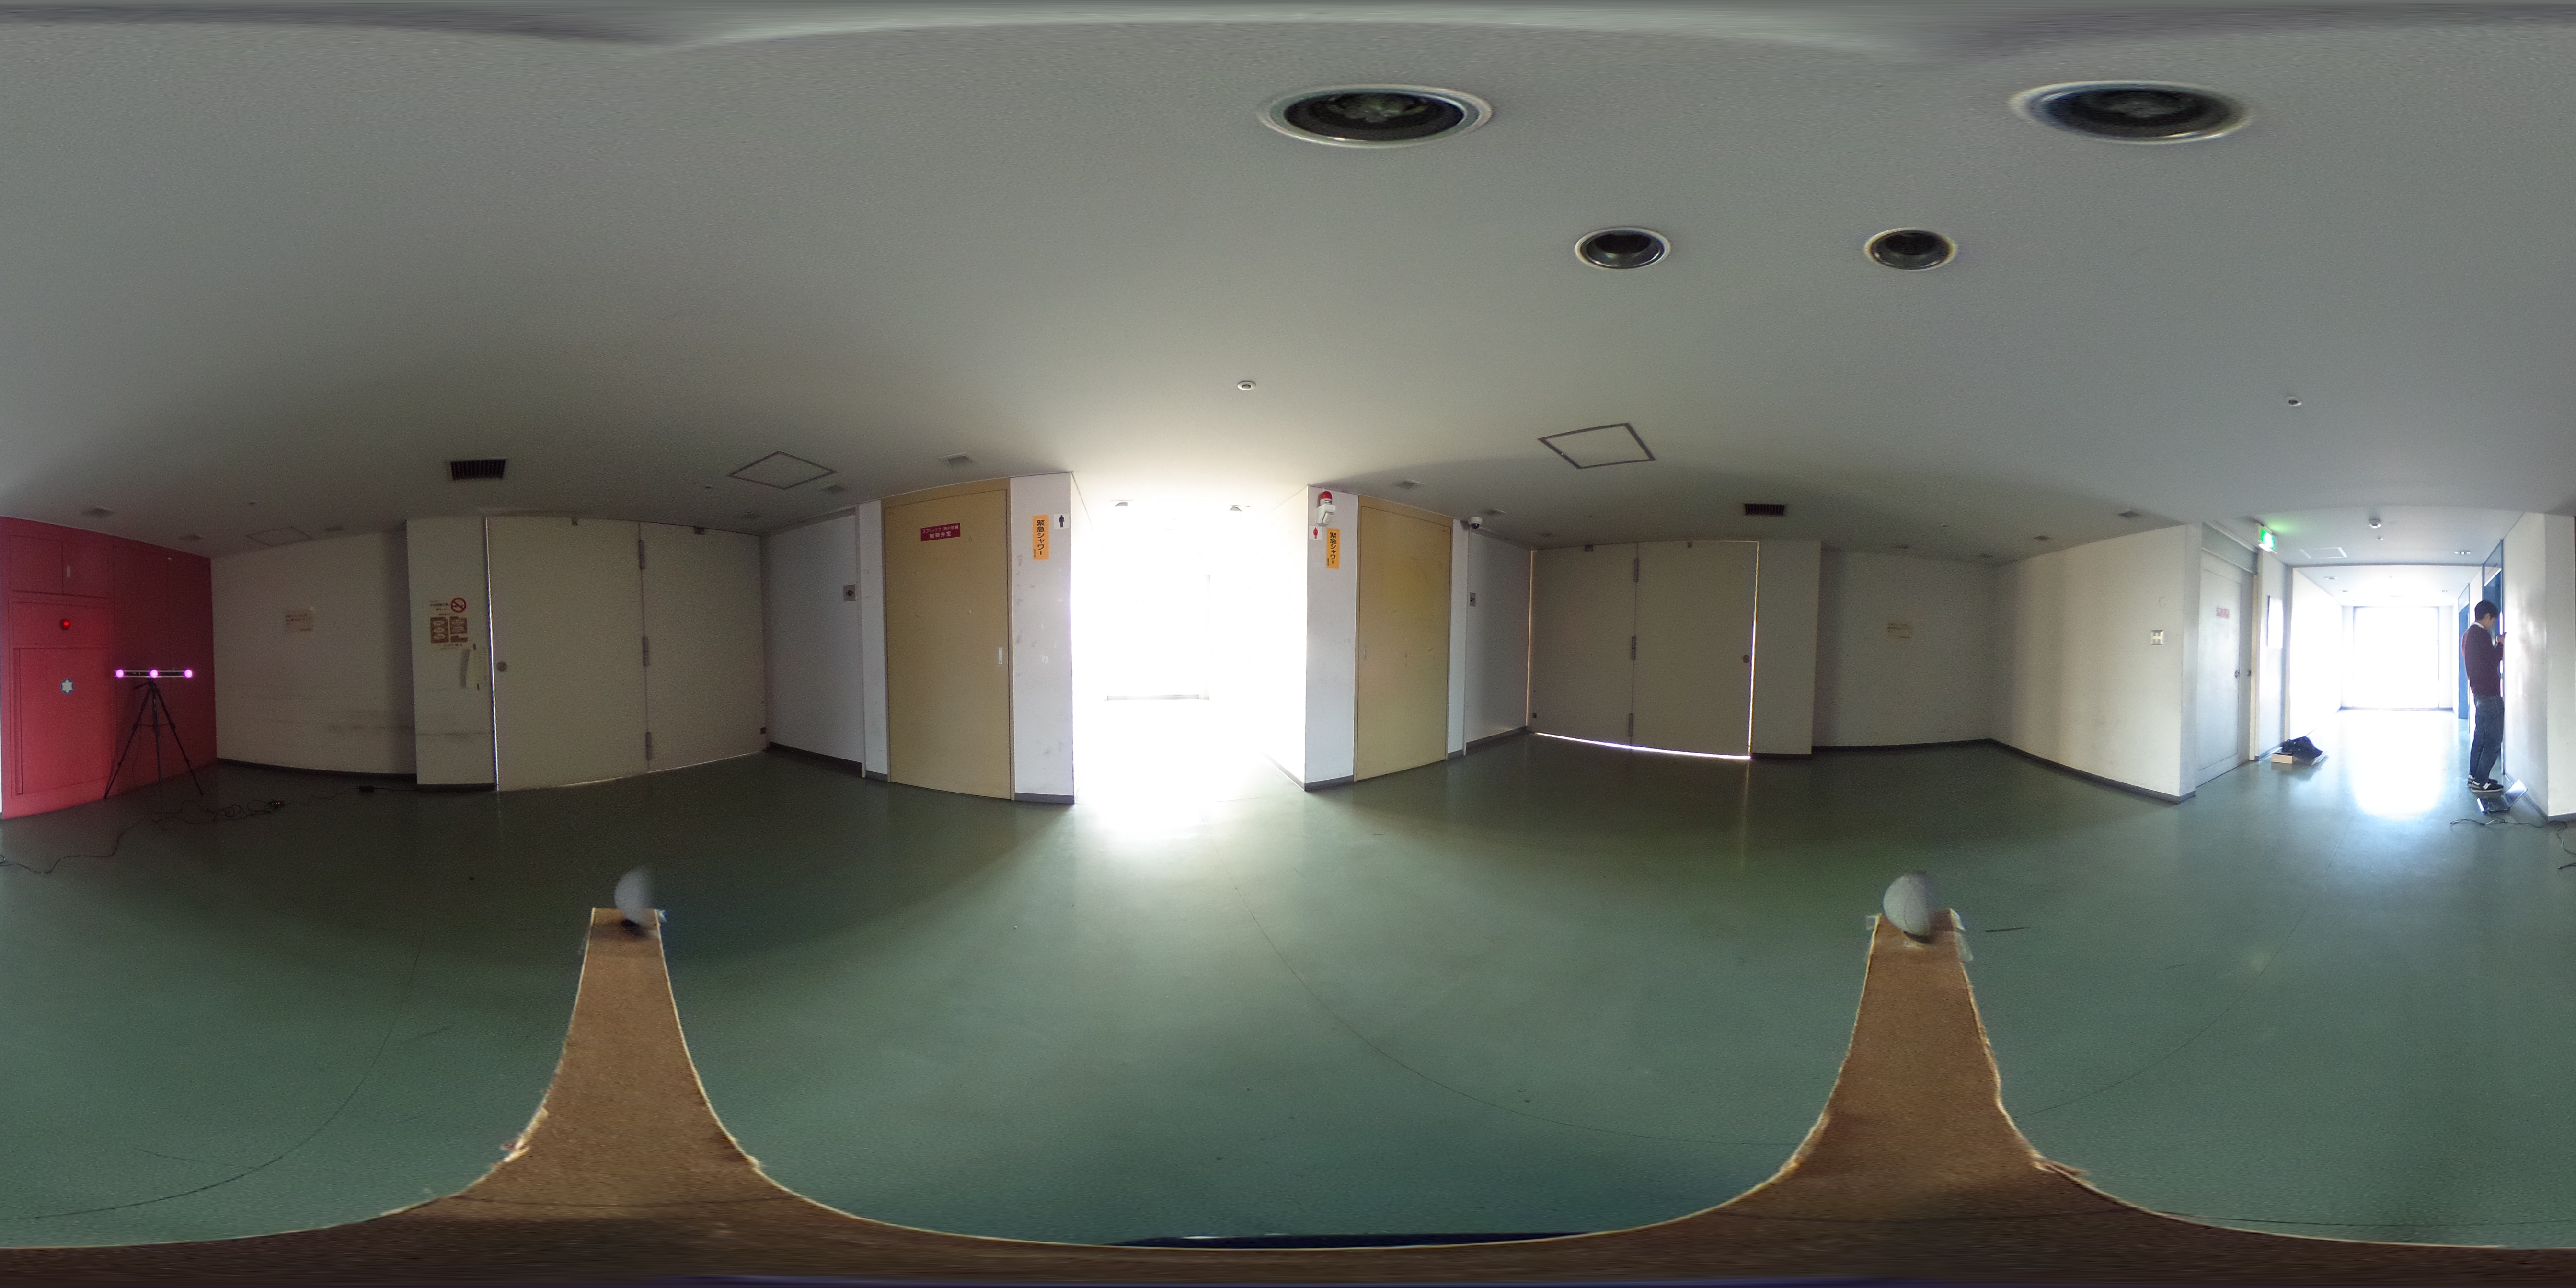
\includegraphics[clip,width=0.45\columnwidth]{./chap5/fig/3.jpg}}
		%\vspace{-5mm}
		\subfigure[地点4]{
		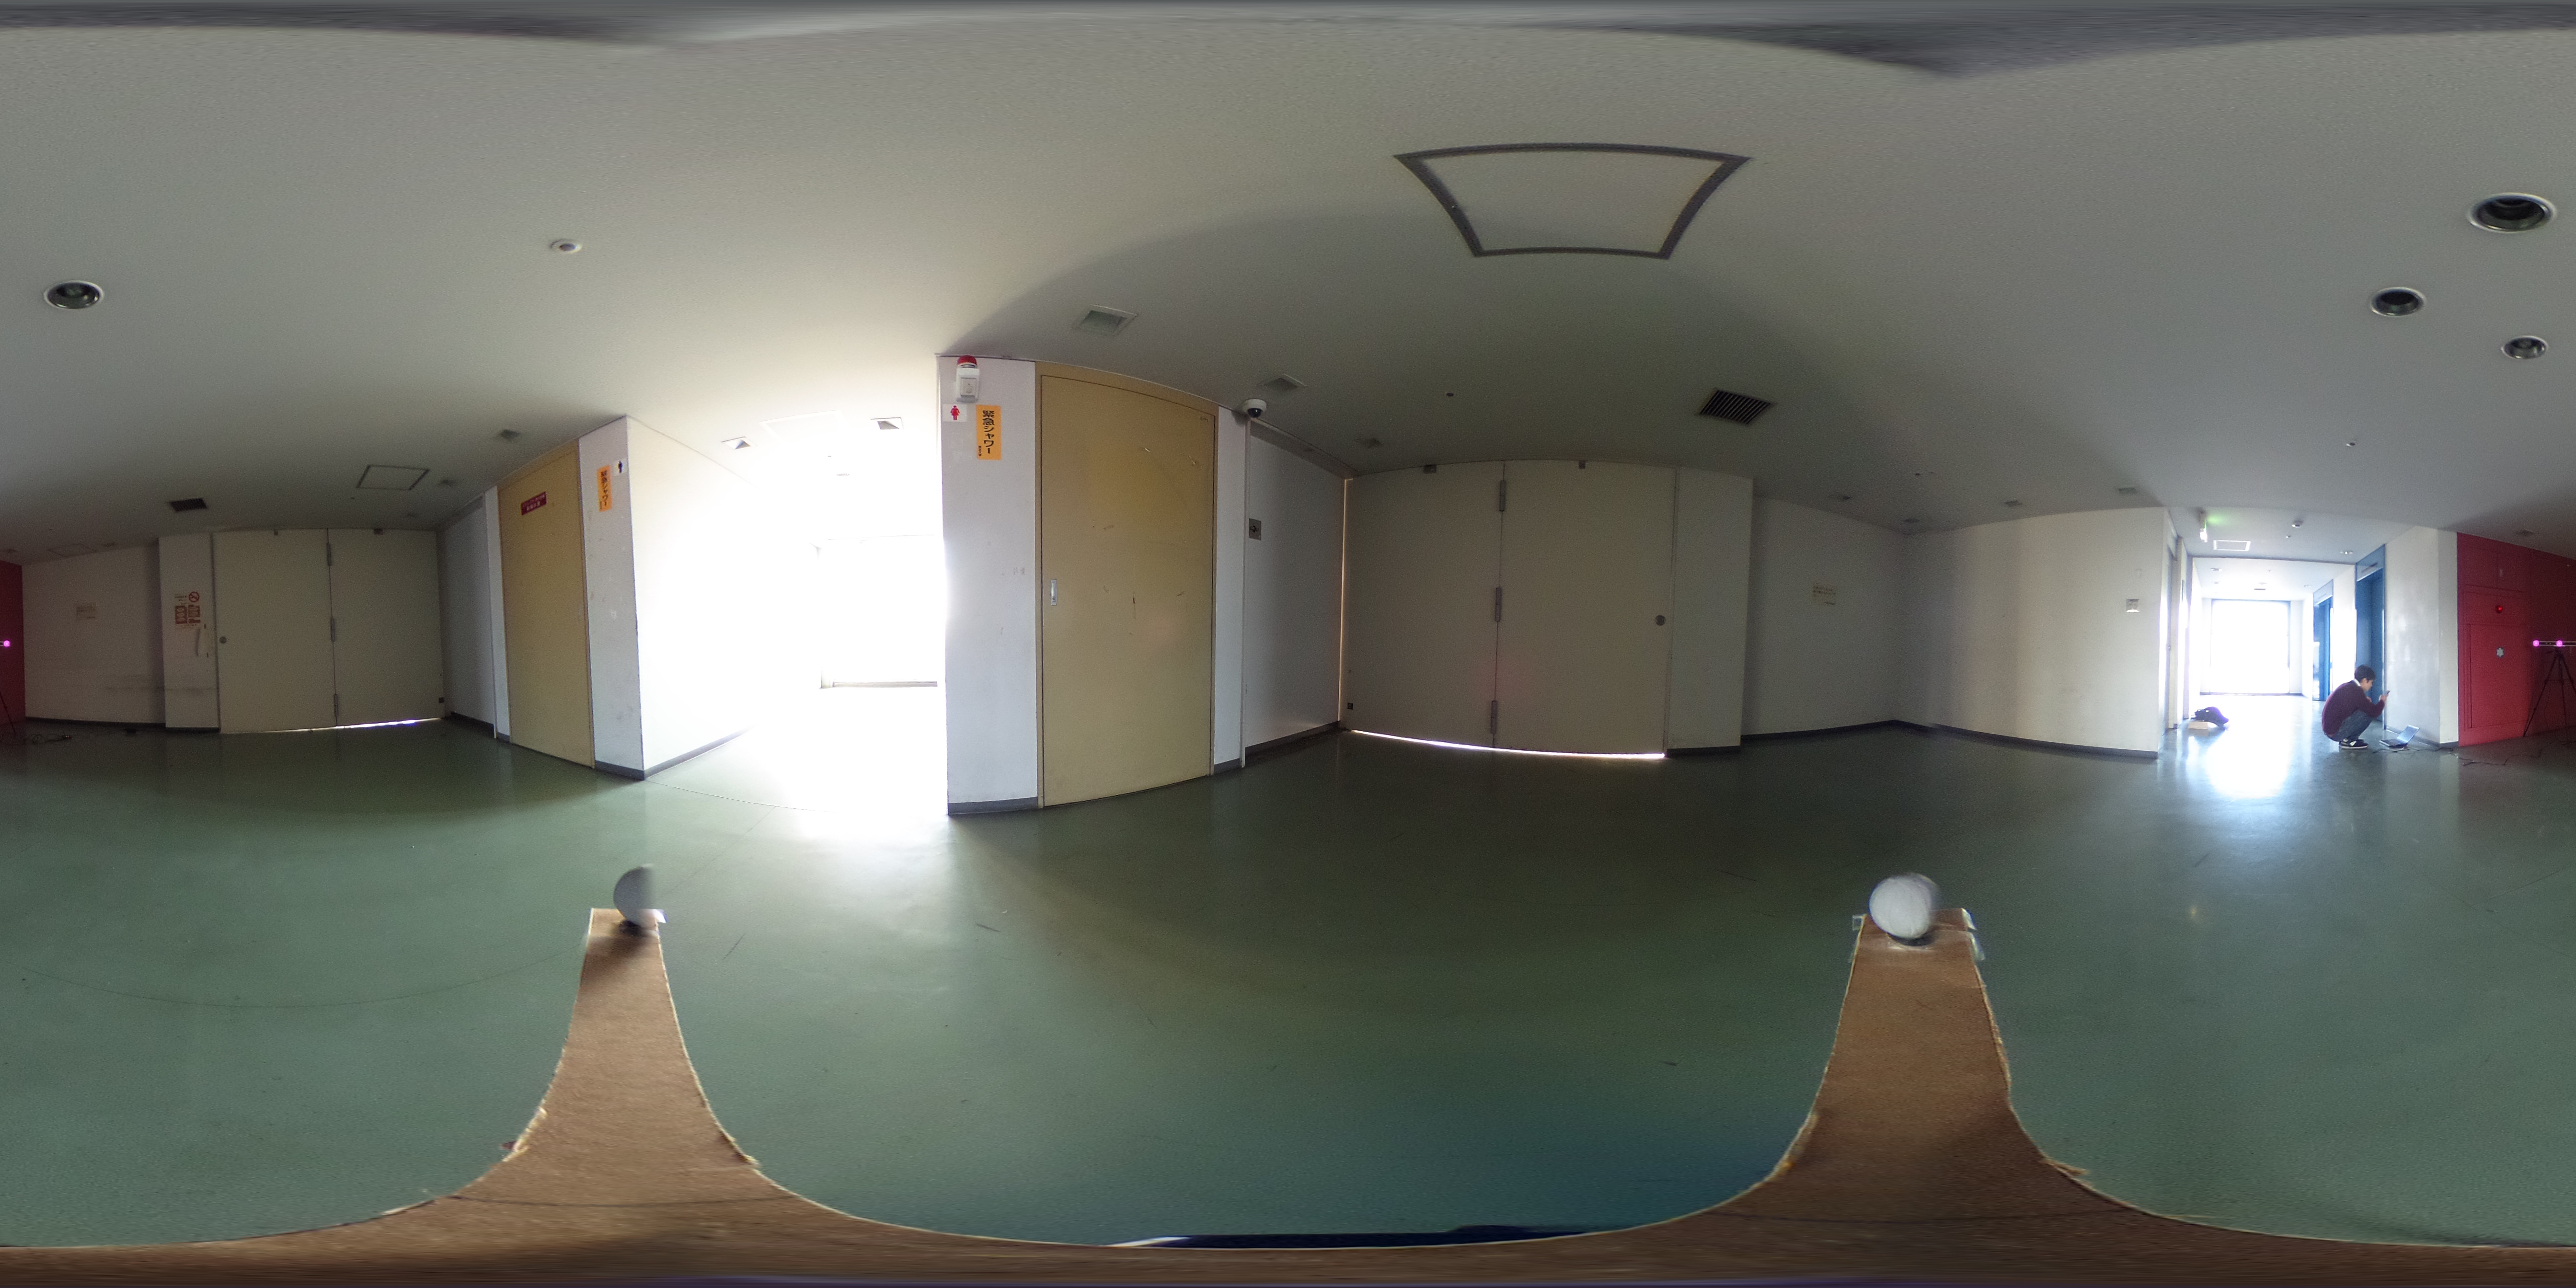
\includegraphics[clip,width=0.45\columnwidth]{./chap5/fig/4.jpg}}\\
		%\vspace{-5mm}
		\subfigure[地点5]{
		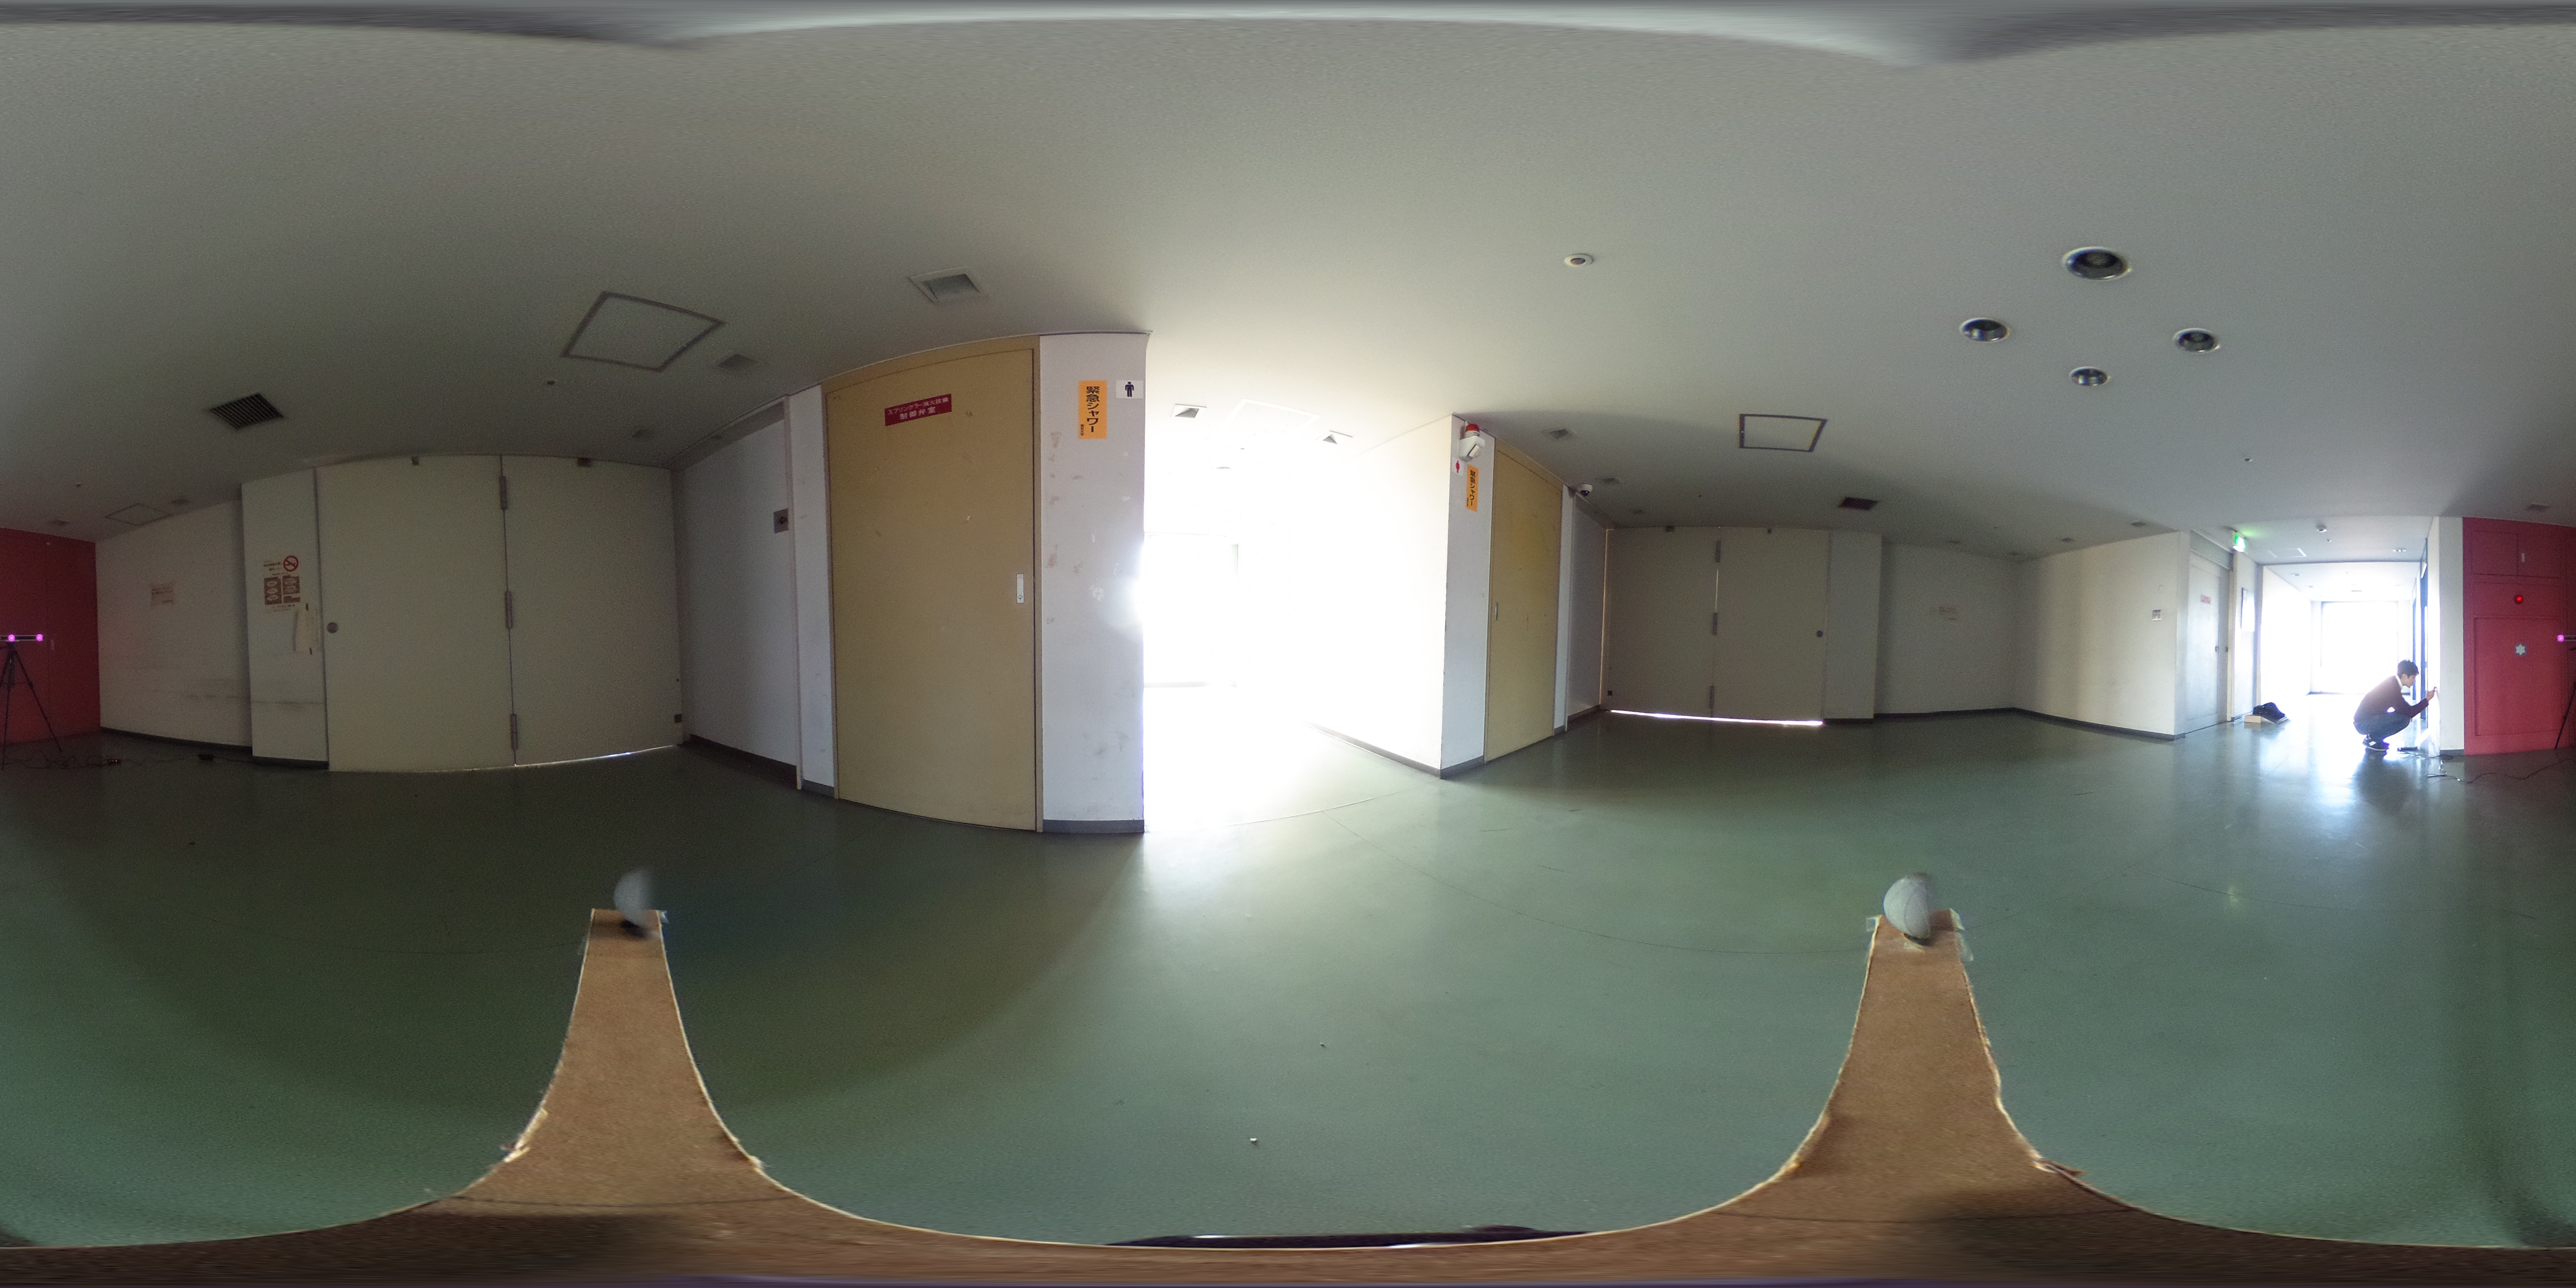
\includegraphics[clip,width=0.45\columnwidth]{./chap5/fig/5.jpg}}
	\caption{5地点における入力画像}
	\label{fig:input_real}
	\end{center}
	%\vspace{-7mm}
\end{figure}

\clearpage
\subsection{結果および考察}

5枚の画像に対する位置姿勢推定に要した計算時間は,2.7$\pm$0.2秒であり,実環境における推定でも高速に推定が可能であることを確認した.
\\

シミュレーション実験と同様にして位置の誤差と姿勢の誤差を計算した結果,各地点における画像の推定誤差は,表\ref{tab:result2}のようになった.
シミュレーション実験と比較して位置,姿勢ともに精度が悪化しており,これは実画像に多く含まれるノイズの影響であると考えられる.

\begin{table}[htb]
 \begin{center}
 \caption{推定誤差}
  \begin{tabular}{c||c|c} \hline
    地点 & 位置誤差 [m] & 姿勢誤差 [deg]  \\ \hline \hline
     1 & 1.83  & 10.1  \\ 
     2 & 1.92 & 7.16  \\ 
     3 & 1.35 & 12.9  \\
     4 & 1.34 & 5.32  \\
     5 & 1.49 & 13.4  \\ \hline
  \end{tabular}
 \label{tab:result2}
 \end{center}
\end{table}


\clearpage
%==============================================================================
%おわりに
%==============================================================================
\section{おわりに}
本章では,提案手法による位置姿勢推定の計算時間,精度,ロバスト性について評価した.

まず5.2節にて,実験の概要について述べた.

次に5.3節にて,シミュレーション環境における実験について述べた.

最後に5.4節にて,実環境における実験について述べた.
\\

提案手法を適用することで,推定精度に関しては課題が残るものの,全天球カメラの位置姿勢を高速に推定できることが確認された.

\newpage
%%%%%%%%%%%%%%%%%%%%%%%%%%%%%%%%%%%%%%%%%%%%%%%%%%%%%%%%%%%%%%%%%%%%%%%%%%%%%%%%
%%%% Local Variables:
%%%% mode: katex
%%%% TeX-master: "../thesis"
%%%% End:
